\documentclass[10pt]{article}

\usepackage{times}
\usepackage[utf8]{inputenc}
\usepackage[T1]{fontenc}
\usepackage[english]{babel}
\usepackage{amssymb}
\usepackage{parskip}
\usepackage{url}
\usepackage{graphicx}

\usepackage{titling}
\setlength{\droptitle}{-1.5in}

\begin{document}

\title{COMP512 - Distributed Systems \\ Deliverable II}
\author{
  Vincent Foley-Bourgon <vincent.foley-bourgon@mail.mcgill.ca> \\
  Carol Morneau <carol.morneau@mail.mcgill.ca>
}
\date{November 2013}

\maketitle


\section{Usage}

All components of the project are launched by using the {\it make}
command with the appropriate task name.  Note that the {\it make}
commands for the RMIs and middleware also start rmiregistry instances
in the background.  Be sure to execute {\it killall -9 rmiregistry}
before you restart the servers.


\begin{verbatim}
$ make runcar    # Start the car RMI
$ make runflight # Start the flight RMI
$ make runhotel  # Start the hotel RMI
$ make runserver # Start the middleware server

$ make runclient # Interactive client
$ make populate  # Automatically load 1000 items in the RMIs
$ make automatedclient # Send random commands to the RMs
\end{verbatim}

\section{Architecture}

\subsection{Lock Manager}

We modified the code in {\it LockManager.java} to accomodate lock
conversion (from read-only lock to read-write lock).  The two methods
we had to modify were {\it Lock} and {\it LockConflict}.  In {\it
  Lock}, if the {\it bConvert} bit is set, we remove the {\it TrxnObj}
and {\it DataObj} from the manager and put in objects with the same
properties, except the {\it LockType} has been changed from read to
write.

In {\it LockConflict}, if the transaction wants a write lock on a data
object and that this transaction already has a read lock, we set the
{\it bConvert} bit to true.  If the transaction already has a write
lock on the data object, we throw a RedundantLockRequest exception.

Every resource manager has a LockManager instance to control access to
its resources.

\subsection{Transaction manager}

The transaction manager is a singleton object inside the middleware
server; it maintains a hash table mapping transaction IDs to a vector
of resource managers.  This allows the middleware to know what kinds
of resources (cars, flights, hotels) a transaction is interacting
with.

The transaction manager also has an {\it isValidTransaction} method
that is called before every RMI call; this is to make sure that all
operations in a valid transaction context.

\subsection{Working set}

The {\it WorkingSet} class allows a transaction to perform different
actions without writing directly into the RMs' hash tables.  A {\it
  WorkingSet} maintains 3 hash maps:

\begin{itemize}
  \item A table mapping transaction IDs to a vector of commands
  \item A table mapping transaction IDs to locations
  \item A table mapping locations to the current state of an object
\end{itemize}

A symbolic representation of the commands sent by the clients is
stored in the first table (no effects occur in the RM at this time).
Once the client commits his transaction, the commands are executed
sequentially, this modifying the state of the RM.  When a transaction
is aborted, the entries for the transaction ID are simply dropped from
the tables.

The two types of commands we store are:

\begin{itemize}
\item {\it CommandPut} describing a write/modify action in a RM's hash
  table
\item {\it CommandDelete} describing a delete action in a RM's hash
  table.
\end{itemize}

During the transaction, a copy of the object is kept in the working
set and modified according to the different commands.  This allows
query operations to see the changed state of the data even though the
updates haven't been committed.

\subsection{Diagrams}

\begin{center}
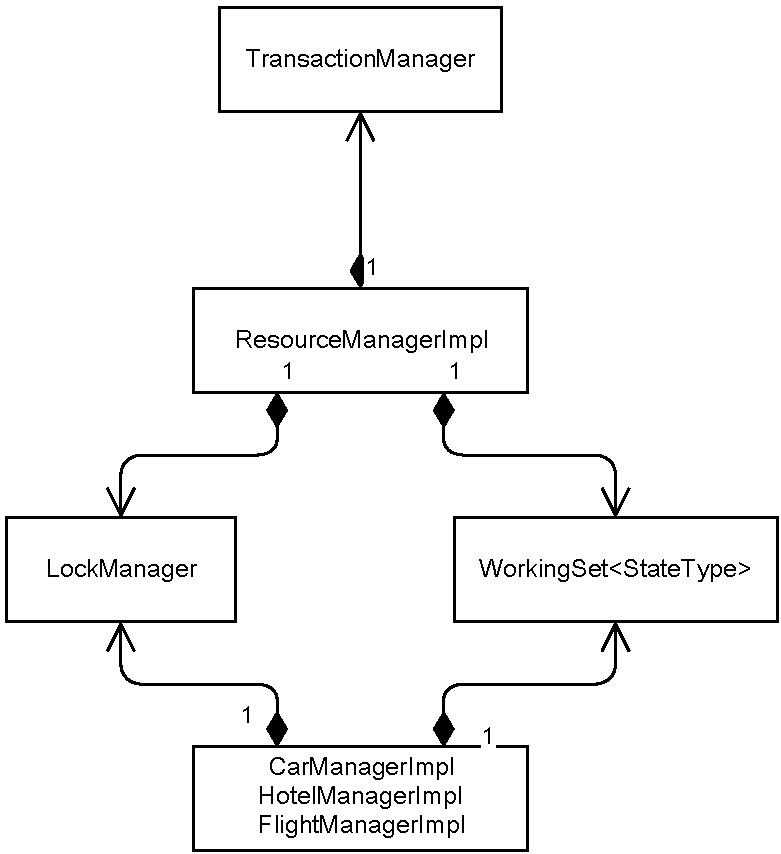
\includegraphics[scale=0.6]{class_diagram.pdf}

~\\~ \\

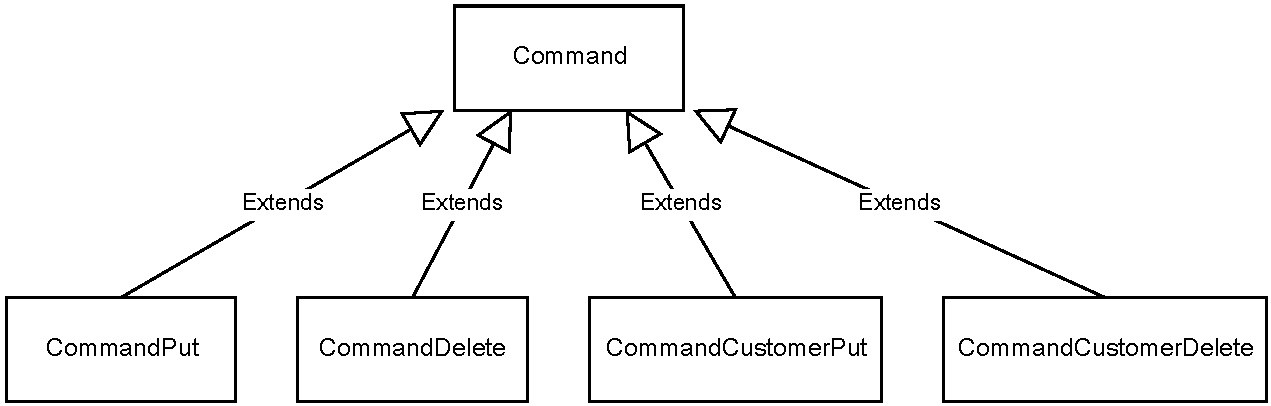
\includegraphics[scale=0.5]{command_hierarchy.pdf}
\end{center}

\begin{center}
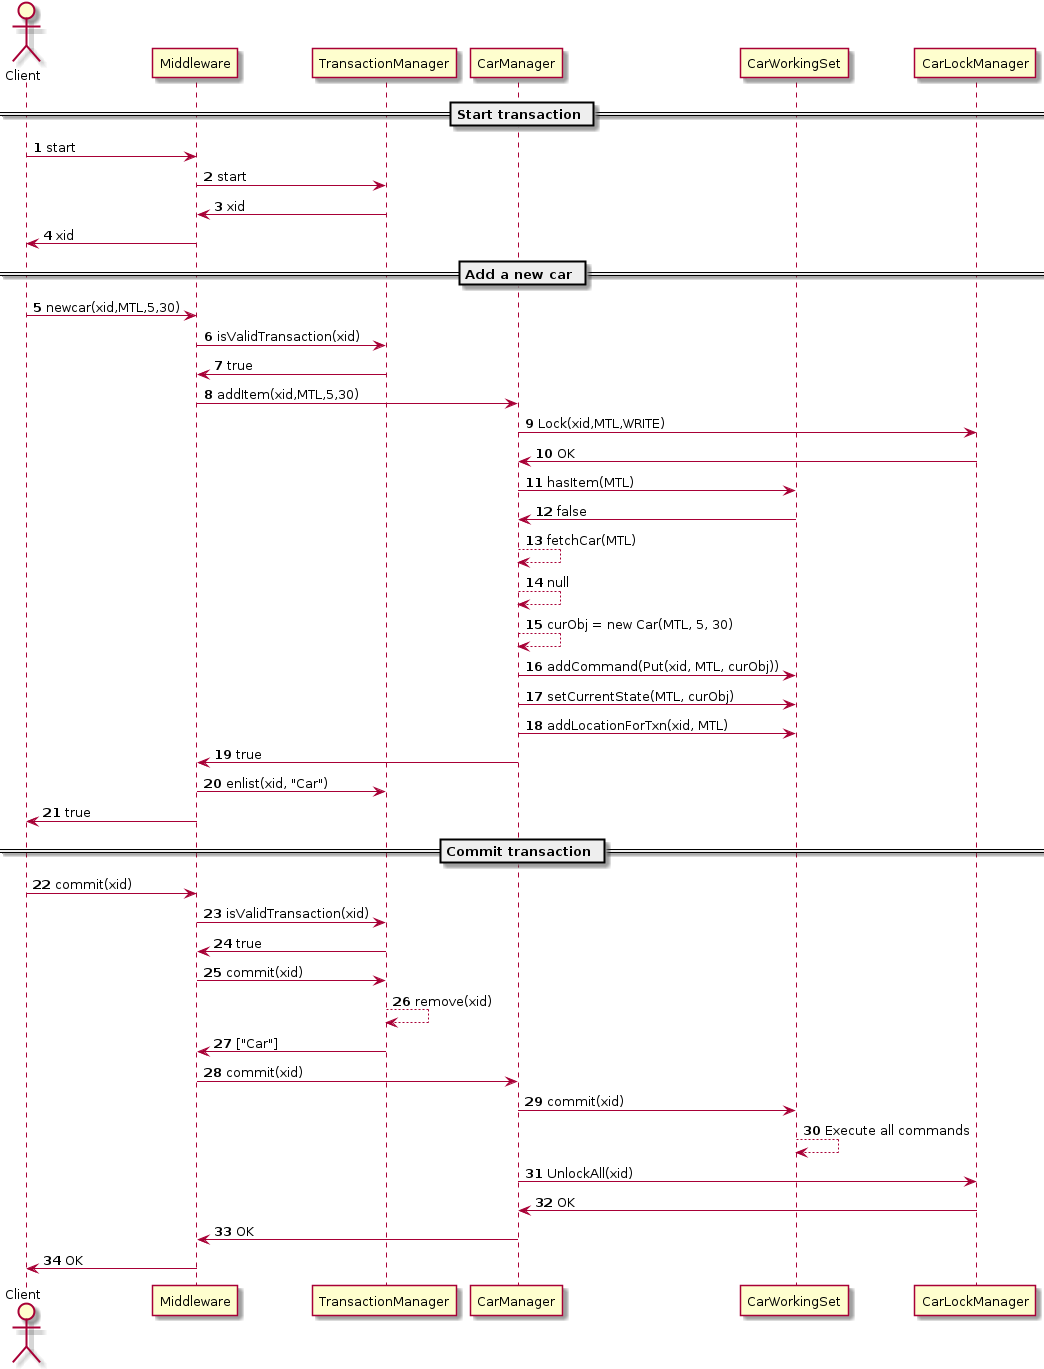
\includegraphics[scale=0.4]{sequence_diagram.png}
\end{center}

\section{Performance evaluation}

\subsection{Single client}

We evaluated the marginal performance of the system by executing read,
write and read/write operations on a single RM and on all three RMs.
We also ended transactions with both commits and aborts.  Because the
times to execute a single command were so low, we executed 50 commands
in total in each transaction.  The average latencies of 1000 measures
are given below in milliseconds.

\begin{tabular}{l|r|r}
  ~ & 1 RM & 3 RMs \\
  \hline
  Read + Commit  & 5.189131 & 6.955100 \\
  Read + Abort   & 5.434654 & 7.042538 \\
  Write + Commit & 12.987475 & 10.064491 \\
  Write + Abort  & 12.985847 & 10.060301 \\
  Read/Write + Commit & 7.466607 & 9.073547 \\
  Read/Write + Abort  & 7.465912 & 9.209547 \\
\end{tabular}

A few surprising facts emerge from these figures:

\begin{itemize}
  \item When only writes are concerned, accessing the 3 RMs is faster
    than accessing only one.
  \item Though they have more work to perform (i.e. executing the
    buffered commands), the commit transactions are usually a little
    faster than the abort transactions.
\end{itemize}

A fact that can only be observed by looking at the raw data is how the
system gets faster as more commands are sent to the system; the first
few transactions execute in ~30ms before reaching numbers usually
below 10ms.  We attribute this to the Java JIT that warms up and
starts optimizing the RM methods after they've been ran a sufficient
number of times.

\subsection{Multiple clients}

For our performance evaluation, we used the following parameters:

\begin{itemize}
\item A fixed number of clients was selected (5, 10, 25, 50, 100, 200,
  500, and 1000)
\item A sleep interval (in milliseconds) between commands was selected
  (1000, 500, 250, 100, 50, 10)
\end{itemize}

For every combination of parameters, the following process was
executed:

\begin{enumerate}
\item The servers were started with empty hash tables.
\item The RMs were populated with 1000 cities (for cars
  and hotels), 1000 flights and 1000 customers.
\item Random commands were executed and committed by the clients for
  60 seconds.
\item The latency times were recorded in a file.
\end{enumerate}

The tests were ran on a Intel i7-3770S 3.10GHz.  To obtain times that
reflected the performance of the application, the server, RMs and
clients were all running on the same machine.  We took the arithmetic
average of the latencies and obtained the chart below.  From this
chart, we can make a few observations:

\begin{itemize}
\item The number of clients has a bigger impact on performance than
  the delay between commands
\item The latency time does not grow linearly with the number of
  clients.
\end{itemize}

Also, not apparent in the chart, the number of deadlocks increased
sharply as the number of clients increased, which is to be expected as
more clients will randomly select the same resource to access.

Finally a chart showing the cumulative distribution function of the
latency times is shown.

\begin{center}
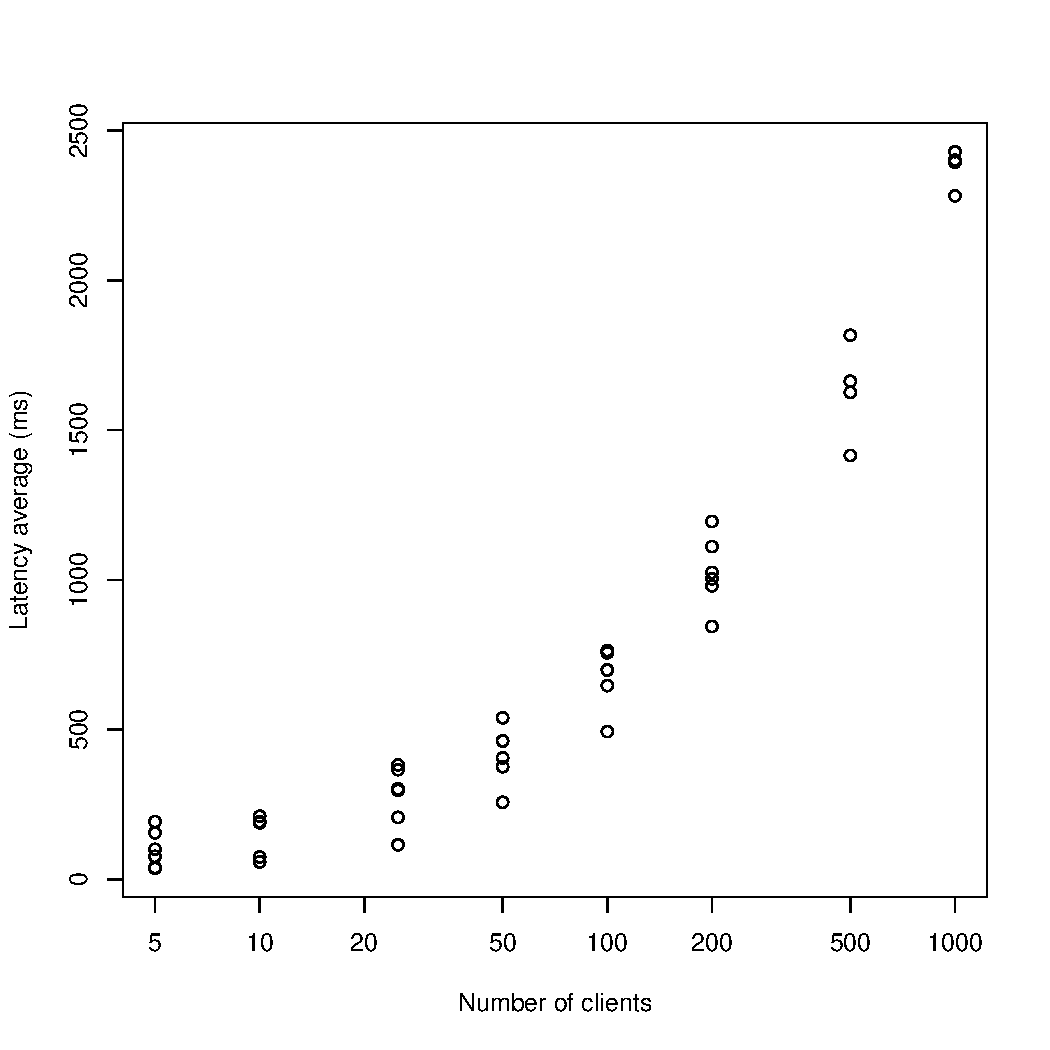
\includegraphics[scale=0.6]{avgs.pdf}
\\
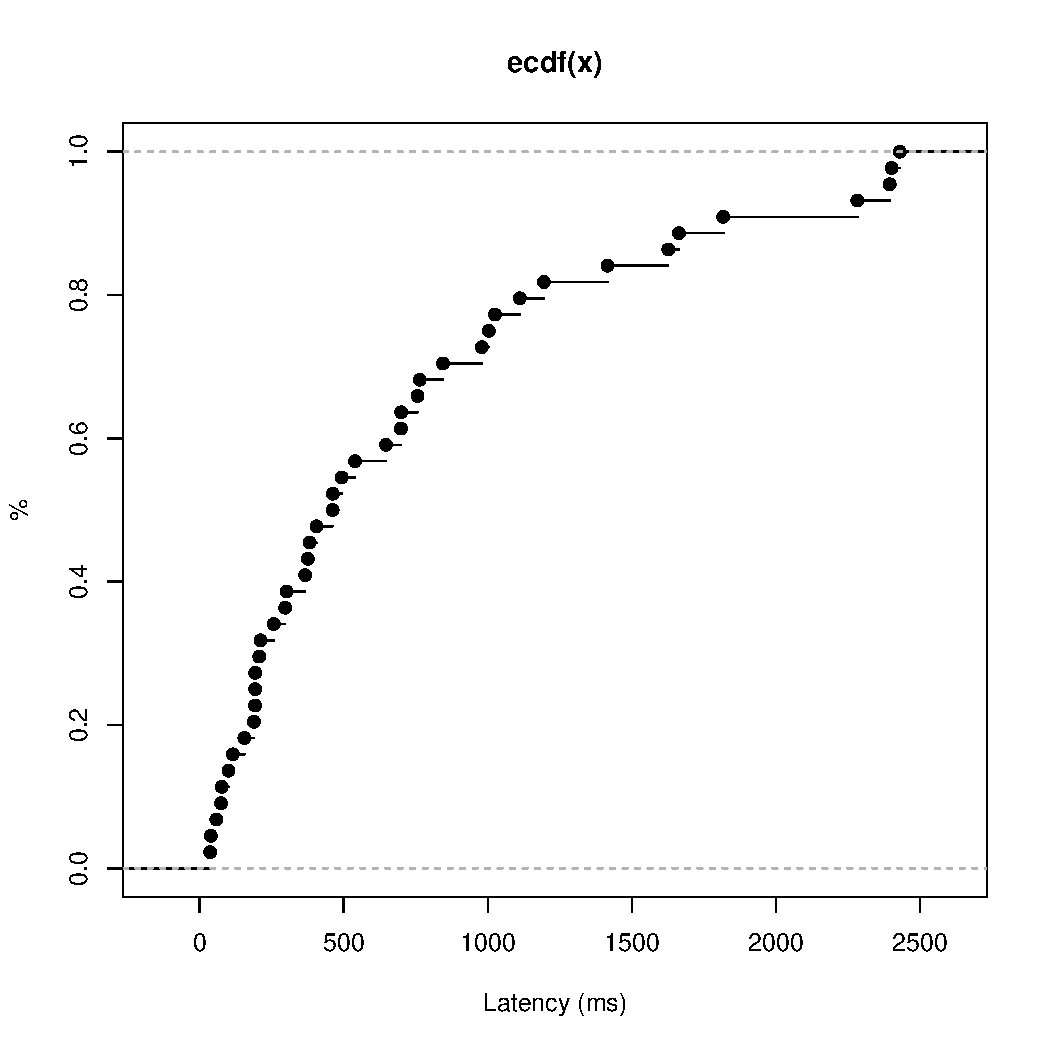
\includegraphics[scale=0.6]{cdf.pdf}
\end{center}


\end{document}
